\documentclass[mim_thesis.tex]{subfiles} 
\begin{document}
The present study was made during the period of January 2018 until March 2018. Due to constant remodeling to improve the user experience and content on openEHR CKM in the last months, several changes may be noticed after the publication of this dissertation.\\

The openEHR Clinical Knowledge Manager (openEHR CKM) was created in April 2009. It is a product from Ocean Health System (ex-Ocean Informatics) and is under the management of the openEHR community. Has become the main international web tool that makes the management of clinical models. The first introduction of CKM had as main objective the creation of an archetype library, development of a review process with achieved content consensus, publication and governance of the artifacts. Since then, the possibility of adding terminology and other terminology specific subsets (SNOMED-CT, LOINC, ICD) has been included. It offers a free registration for individuals from all around the world, focused on giving added value to the repository on a voluntary basis. All non-technical health care area professionals are also encourage to contribute, is not a requirement to be a physician to redound. Is possible to purpose new artifacts (archetypes, templates), suggest corrections and participate in discussions, translate archetypes to other languages, watch or adopt archetypes. All the changes to an archetype are subjected to a consensual decision from all reviewers before being published. The CKM has a model governance system that supports all the life cycle of archetypes, templates and terminology. In 18 January 2018, it contained 1840 users and 679 archetypes (respectively 11,8 and 4,1 times more than May 2009 \citep{conde2010towards}. This growing up stand is only possible due to having an active online community that is working together on determine clinical definitions. 

\begin{figure}[H]
	\centering
    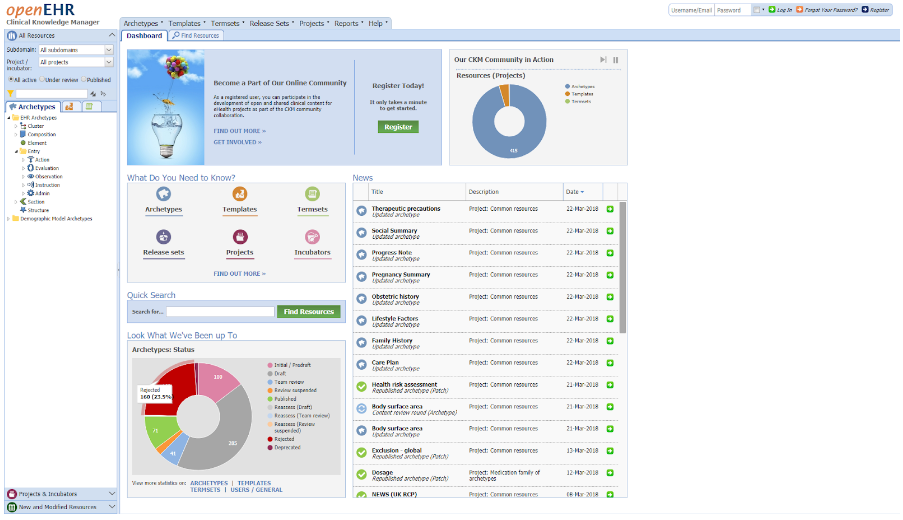
\includegraphics[width=0.7\textwidth]{img/openehr_ckm.PNG}
	\caption{OpenEHR Clinical Knowledge Manager (March 2018)}
	\label{fig:openehr_ckm}
\end{figure}

\section{Instances of CKM}
Inasmuch as there are different requirements between different countries or even projects, others instances of CKM for national registries had been made, such as Norwegian Nasjonal IKT CKM, Australian Digital Health Agency CKM, NHS England CKM, Shared UK CKM (Apperta Foundation, Scottish Government) and the Slovenian MoH CKM. The following table presents the active national and international CKM instances available.

\begin{table}[H]
\centering
\caption{ List of active openEHR related software and modelling tools (march 2018)}
\label{tab:tools}
\begin{tabular}{p{1.5cm} p{3cm} p{2cm} p{3cm} p{1.7cm} p{3cm}}
\toprule[2pt]
\textbf{Name} & \textbf{Description} & \textbf{Publisher Organization} & \textbf{Publisher Namespace} & \textbf{Primary Language}  & \textbf{Git Repository}                                                         \\ \midrule[2pt]
\textbf{openEHR CKM}  & The CKM for the international openEHR community. & openEHR Foundation  & org.openehr & English & \url{https://github.com/openEHR/CKM-mirror}                                                       \\ \midrule
\textbf{Australian Digital Health Agency CKM} & Hosted by Australian Digital Health Agency for the Australian national digital health program & Australian Digital Health Agency & au.org.nehta & English &\url{N/A} \\ \midrule
\textbf{UK Clinical Models / Apperta CKM} & The CKM for resources developed collaboratively within UK projects. & UK Clinical Models / Apperta Foundation & uk.org.clinicalmodels & English & \url{https://github.com/ClinicalModelsUK/ckm}       
\\ \midrule
\textbf{Norwegian CKM} & Hosted and managed by the Norwegian national eHealth program.                        & Nasjonal IKT & no.nasjonalikt & Norwegian & \url{https://github.com/Arketyper-no/ckm}      
\\ \midrule
\textbf{Slovenian CKM} & Hosted and managed by the Ministry of Health in Slovenia. & si.ezdrav & si.ezdrav & Slovenian & \url{N/A}                                                         
\\ \midrule
\textbf{Alberta CKM} & Hosted by the Canadian Alberta Health Services  & Alberta Health Services, Canada  & ca.ahs & English & \url{N/A}                                           
\\ \midrule
\textbf{CKM Test server}  & Hosted by Ocean Informatics for testing and demoing purposes & Ocean Informatics  & com.oceaninformatics & English & \url{N/A}                           
\\ \bottomrule[2pt]
\end{tabular}
\end{table}

These instances are totally independent from each other. The archetypes inside of each instance can differ with the related use case and even when making an user registration/account in one domain, this account will not be created or replicated in the other domains.

\section{Roles}
OpenEHR CKM offers three levels of management roles \citep{openEHRCKM}:
\begin{itemize}[noitemsep]
\item Systemwide; 
\item Subdomain; 
\item Project/incubator.
\end{itemize}

The international openEHR (main domain) is ruled by the systemwide role. This role also offers a different case of sub-roles as administrators: “\textit{Clinical Knowledge administrator}” and “\textit{Technical administrator}”, that gives complete rights for CKM administration, although notifications can differ between both. Then, there are other sub-roles like “\textit{classes modifier}”, “\textit{classifications modifier}”, “\textit{scheme modifier}”, “\textit{scheme translator}” and “\textit{release set modifier}”. 

The other role is located in the subdomain level, called the “\textit{subdomain admin}”, that manages one of the instances from OpenEHR CKM, the national domains: Norwegian CKM, UK clinical models, NEHTA CKM or Alberta Health Services. In the case of project/incubator level the roles are “\textit{editor}” and “\textit{reviewer}”.

When a user makes his own registration on the OpenEHR CKM, a normal user role is assigned to him. Then, is possible for the user to define what is his health domain and profession. Depending on the provided info, he can be part of the upper role levels. Also a “\textit{normal user}” is not assigned to any of those roles mentioned before and can review artifacts that are not owned by any other project or incubator. 

\section{Features and functionalities}
Despite of being a repository for OpenEHR artifacts, where it is possible to upload or download these contents, the CKM has another functionalities. For a guest, he can search archetypes, templates or term sets in the international repository, including as well the others national instances and projects. Also there is the possibility to check analytical and statistical data on the repository, including total number of uploaded archetypes, information of registered users (professional status, world distribution), last uploaded and updated artifacts and projects, and give bug reporting in case of malfunction of the repository. The CKM offers free user registration and those accounts can have different roles, that were already mentioned above. Is possible as a registered user to purpose and submit creations or changes of archetypes that will be reviewed by the OpenEHR community, join projects and create incubators, set preferred views of subdomains (e.g. national instances) and respective projects/incubators, download archetypes or templates with draft and published status, make language translations of the artifacts with the possibility of watch and adopt them and participate in content discussions. 

One of the most interesting features is the way the information of the chosen archetype or template is shown on the CKM and how it is possible to manage them. After searching and open an archetype, if the user has an account, a special kind of toolbar is associated to it. This toolbar has various options and views that can be suitable for a different type of users - a healthcare professional would prefer to see the structure of an archetype in a mindmap view and a informatician would prefer to see that as an XML file. The available information views are the tabbed view, mindmap and XML. Each one of them gives information about the header, attribution, data, state, protocol, pathway, related events and the respective reference model associated to that archetype. The header, only available in the tabbed view, contains the specific content like the concept name associated and respective description, keywords, purpose of the archetype, information about use and misuse of that content, other additional identification (build UID, major version ID, MD5 hash), authors and contributors (editors and translators). 

\begin{figure}[H]
	\centering
    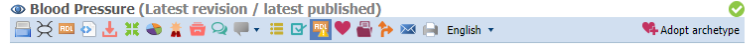
\includegraphics[width=0.9\textwidth]{img/editor_resource_toolbar.PNG}
	\caption{Editor resource toolbar (registered user version) }
	\label{fig:editor_resource_toolbar}
\end{figure}

Other interesting section is “archetype history”, which offers all the historical information from the selected archetype, being possible to see all the changes that affected the content development in each trunk and respective branches (resolved, outdated, committed and active) of the repository. Each committed branch to the trunk was done after consensus by all the openEHR reviewers team. If new changes are necessary, new branches can be open in the new version of the trunk. It is also possible to check and download the previous versions of the current archetype. The section “related resources” give information about where the archetype is being used, in which templates are inserted, the parent and children relationships from it and if there is any predecessor or successor for this archetype.  

\begin{figure}[H]
	\centering
    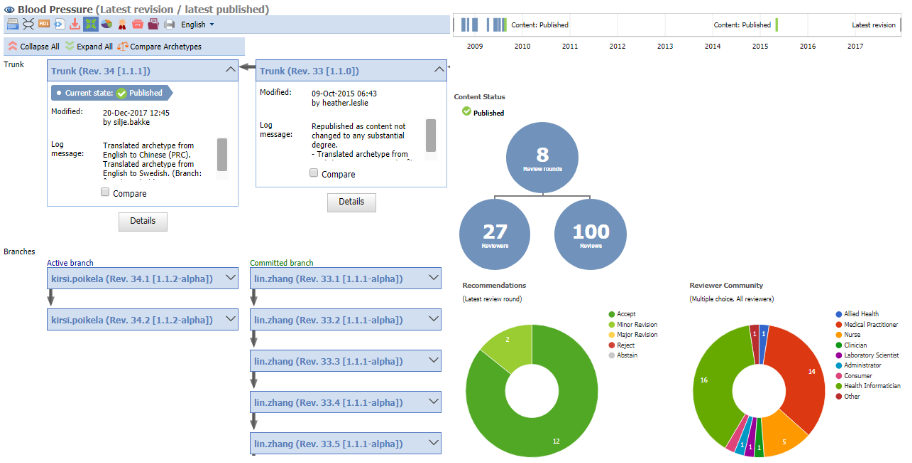
\includegraphics[width=0.95\textwidth]{img/bp_history.PNG}
	\caption{ Blood Pressure archetype historical information and status (march 2018)}
	\label{fig:bp_history}
\end{figure}

Also on this toolbar, there is an analytical view, called “Status” that gives information about how is the current status of the archetype (Initial/pre-draft, draft, review suspended, team review or published), how many reviews rounds, reviewers and total reviews were involved, recommendations from the latest review round, the background of reviewers community, terminology and translation status. With all the functionalities mentioned, it is possible to conclude that the possibility of having an online community working together on this web tool can give an added value to the improvement of health care IT, since it can decrease time and costs between the face-to-face meetings, it provides online versioning management and mutual revision with discussion.


\section{Management of artifacts}

All the management made with the artifacts are directly done in the openEHR CKM or in the other instances. Depending on the user role, openEHR CKM offers a model that allows to made easily changes and updates on a archetype by revising it. For that, a "branch" can be created for the revision, where is included the information of who has created the submission and a log message with information related with this branch. During all the steps of revision, the artifact will be check by health informaticians or analysts until getting a full agreement between all. 

The archetypes usually have six stages in the management cycle. They are created if there is a clinical need, shared in a web based repository, reused on a different templates templates among various EHR systems, specialized in case of a specific clinical need (e. g. weight to child-weigh), revised in case of an error on the archetype that needs to be corrected and updated and versioned when the core archetype (the root archetype) is having flaws and needs to be remodeled. \citep{article2006leslie}


\section{Identifying parameters of new versions of archetypes}

OpenEHR has dedicated a section that takes care of versioning of archetypes and templates, called the \ac{AOM}, a package inside on the \ac{AM}. In this section will be explained how this package works and what are the inherited parameters from another packages in the OpenEHR Reference Model, which and what are the parameters for version controlling and how to identify in a human and machine readable way the identification of each archetype, associated to his governance and life cycle. 

\subsection{The Archetype Object Model (AOM)}
The AOM is a programming object from Archetype Model (AM) \citep{openEHRAOM}, that contains all the variables and parameters related with  archetype and template identification, such as archetype specialization, authoring of archetypes, version numbering and respective modifications. Currently, it goes in the version 2, after being renamed from version 1.5 and includes extensions made from the version 1.4 of the ADL, like meta-data, new internal coding system, terminologies addition and many others. \par 
These archetypes parameters are under the ARCHETYPE\_HRID and AUTHORED\_ARCHETYPE classes (that has inherited classes and parameters from the RESOURCE package), which can be seen the figure \ref{fig:RM_archtype}, represented by a \ac{LDM} for the AM package. Archetypes have two ways defined to be understood by machines or by humans \citep{openEHRarchver}. The human way is called Human readable Identifier (HRID), which consists on an identification structure that is defined by the ARCHETYPE\_HRID class. Inside of this class, there are parameters defined for each part of the "full" archetype name.

\begin{figure}[H]
	\centering
    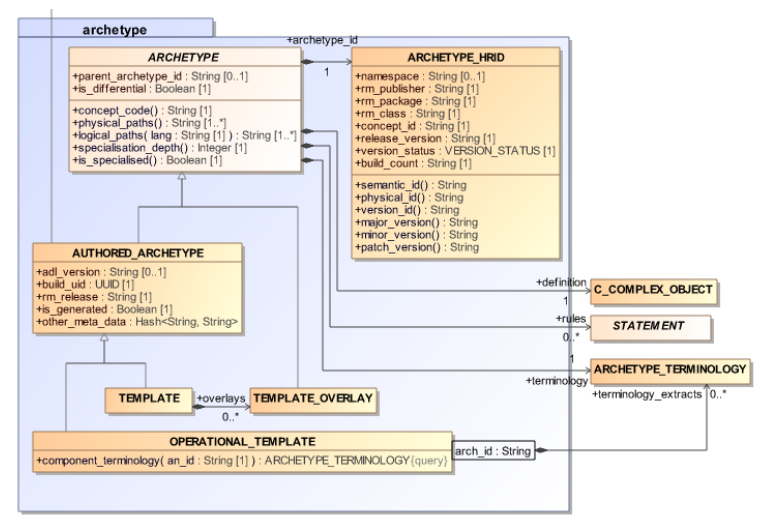
\includegraphics[width=1\textwidth]{img/RM_archtype.PNG}
	\caption{am.aom2.archetype Package (from openEHR Archetype specification) MUDAR IMAGEM PARA VERSAO COMPLETA}
	\label{fig:RM_archtype}
\end{figure}

This archetype name can be sorted in two ways, one by \textit{semantic\_id} which contains the extension of version status and the build\_count that shows the development status of that archetype, or by the \textit{physical\_id}, which is the formal aspect of an released archetype. This structures are composed by: \\

\textbf{Structure for \textit{semantic\_id:}} 

\textit{namespace::rm\_publisher-model\_name-
rm\_class.concept\_id.v.major\_version.minor\_version.patch\_version-
version\_status.build\_count}
\begin{itemize}[noitemsep]
\item Case example:
\begin{itemize}[noitemsep]
\item org.openehr::openEHR-EHR-OBSERVATION.blood\_pressure.v1.0.5-rc.17 
\item org.openehr::openEHR-EHR-OBSERVATION.blood\_pressure.v1.0.5-alpha \\ 
\end{itemize}
\end{itemize}

\textbf{Structure for \textit{physical\_id:}} 

\textit{namespace::rm\_publisher-model\_name-
rm\_class.concept\_id.v.major\_version.minor\_version.patch\_version}
\begin{itemize}[noitemsep]
\item Case example:
\begin{itemize}[noitemsep]
\item org.openehr::openEHR-EHR-OBSERVATION.blood\_pressure.v1.0.5
\end{itemize}
\end{itemize}

If dividing all the parameters from the \textit{semantic\_id}, to match each parameter inside of the ARCHETYPE\_HRID class, they can be filled up as: 
\begin{itemize}[noitemsep]
\item \textbf{namespace:} org.openehr
\item \textbf{rm\_publisher:} openEHR
\item \textbf{model\_name:} EHR
\item \textbf{rm\_class:} OBSERVATION
\item \textbf{concept\_id:} blood\_pressure
\item \textbf{release version:} 1.0.5
\begin{itemize}
\item \textbf{major\_version:} 1
\item \textbf{minor\_version:} 0
\item \textbf{patch\_version:} 5
\end{itemize}
\item \textbf{extension:}
\begin{itemize}
\item \textbf{version\_status:} "rc" or "alpha"
\item \textbf{build\_count:} 17
\end{itemize}
\end{itemize}

The junction of each one of these parameters lead to the full identification of the archetype in a human readable way. The machine readable way is composed by the MD5-CAM, archetype\_uid and build\_uid. Is possible to affirm that "\textit{ARCHETYPE.archetype\_id.semantic\_id}" is the equivalent readable human way of the \textit{"ARCHETYPE.uid"}, a machine identifier.\\


\subsubsection{Version numbering}

In the specifications for archetype versioning and identification \citep{openEHRarchver}, the \textbf{"revision"} parameter has special rules for the numbering identification based on \textit{semVer} standard. The first three levels on numbering are identified by dot-separated numeric parts (\textit{majorVersion.minorVersion.pathVersion}). 
The \textit{majorVersion} is incremented when there is a major and significant change to the artifact formal definition. This significant change can be the removal of mandatory data points or groups, removal of nodes (also known as paths), move of those nodes to different sub-tree or the change of domain definition of id-code. The \textit{minorVersion} is characterized by a lesser change such as changes in the constraints, including node RM types, additional definition nodes (e.g. new paths) or the addition of terminology bindings. In the case of \textit{patchVersion}, this is incremented each time there is an informal change of the archetype formal definition like changes to meta-data, addition of language translations, changes to wording of terminology that do not affect the sense of the definition or when the archetype is rejected. \citep{openEHRAOM_AIS} \par
These three levels can be identified as "\textit{release\_version}" and this identifier can have added an extension including the (\textit{versionModifier.issueNumber}) which gives the information about the \textbf{"lifecycle status"} and the current build number / issue number. The lifecycle status can be composed by an alpha element ("-alpha") for an "under development" or "unstable" archetype and a "release candidate" ("-rc") for a archetype with a pre-release version. For example, it is possible to have two different types of revision parameters based on the previous explanation:

\begin{itemize}[noitemsep]
\item \textbf{1.1.1-rc.12} , translated from (\textit{release\_version-description.lifecycle\_state.build\_count}) and it means that has a 3 part version identifier and is a release candidate with the build count of 12, which is incremented in every commit.
\item \textbf{1.1.0-alpha} , translated as (\textit{release\_version- description.lifecycle\_state}) and is an archetype with a alpha development version based on 1.1.0 version. 
\end{itemize}

An example of a archetype life cycle containing the \textit{release\_version-description.lifecycle\_state} can be: 
\begin{center}
{1.1.5-rc.1 < 1.1.5-rc.2 < 1.1.5 < 1.1.6-alpha < 1.2.0-alpha < ... < 1.2.0}
\end{center}

The major version is reflected on the HRID source identifier, by ending the "archetype\_id" (e.g. openEHR-EHR-OBSERVATION.blood\_pressure.v1) with "v.X", being X the value from the \textit{majorVersion}. In the first version of the archetype, the  \textit{majorVersion} always starts with zero, having the "revision" parameters as (0.0.1). The identification name for an archetype with this parameters is "openEHR-EHR-OBSERVATION.blood\_pressure.v0" (\textit{RM\_publisher-RM\_closure-RM\_class-concept\_id.vX}).

The lifecycle status have specials names to map the classification of an archetype:
\begin{table}[H]
\caption{Archetype lifecycle mapping (XML format)}
\label{tab:arch_lifecycle_xml}
\centering
\begin{tabular}{l}
\toprule[2pt]
\begin{lstlisting}[language=XML]
aom_lifecycle_mappings = <

	["AuthorDraft"] = <"unmanaged">
	["Draft"]	= <"in_development">
	["TeamReview"] = <"in_development">
	["Team Review"] = <"in_development">
	["ReviewSuspended"] = <"in_development">
	["Review Suspended"] = <"in_development">
	["Reassess"] = <"published">
	["Published"] = <"published">
	["Rejected"] = <"rejected">

>
\end{lstlisting}
\tabularnewline \bottomrule[2pt]
\end{tabular}
\end{table}


NOTA: - as vezes as diferencas sao praticamente nulas, pode ser a correcao de uma palavra, ou adicionar o lifecycle, o que vai fazer com que toda a informacao do MD5 mude. as vezes ate pode nem mudar, mas a juncao do md5 com uid e revision dá para ter a ideia de que algo mudou.

TODO \url{http://www.openehr.org/releases/AM/latest/docs/Identification/Identification.html#_need_for_rm_class_name_in_identifier}
---------- Isto vai servir para explicar o AOM no adl designer.\\
COLOCAR MAIS ALGUMA COISA AQUI

\subsubsection{Versioning parameters inside of ADL files}

An EHR based on openEHR can digitally sign every version of an artifact in a versioned object (e.g. encounters). This artifacts are signed with a digital signature, composed by a private key encryption (RSA) of a hash (MD5) from the canonical representation of that versioned file (e.g. XML schema), using the openPGP message format. When the artifacts undergo with updates, these acts are called as contributions. Each contribution is then marked inside of the archetype with an attributed identification and integrity parameters mentioned above (MD5, build\_UID), that allows for each archetype to have a unique way to be managed in case of further changes. These parameters are based on cryptographic hash algorithms, which aim is to transform one input of variable size in an output of lesser and fixed size. For example, all the information of an archetype can be inserted in a hash like “7341F7E8A07ACE883A5F541BA79F2B95”. These algorithms are non-injective functions and the output identification of each of them can not be unequivocal. That means that some messages can have the same hash string and if they have the same hash, the input message should be equal on both, but it should not be possible to retrieve the original message by decrypting that hash. 

Relating this with the openEHR artifacts, an archetype with the same hash value of the item "MD5-CAM 1.0.1" should have the same information in the XML and ADL body. The identification parameters for the openEHR archetypes are shown in the table \ref{tab:bp_xml_adl}.

\begin{table}[H]
\caption{Excerpt from blood pressure archetype (XML and ADL format)}
\label{tab:bp_xml_adl}
\begin{tabular}{l}
\toprule[2pt]
\begin{lstlisting}[language=XML]
XML:    
      (...)
      <uid>
        <value>b1506a87-9bf2-4978-9eed-6ceecb0c2be9</value>
      </uid>
     <archetype_id>
       <value>openEHR-EHR-OBSERVATION.blood_pressure.v1</value>
     </archetype_id>
       <adl_version>1.4</adl_version>
      (...)
         <lifecycle_state>published</lifecycle_state>
      (...)
        <other_details id="original_namespace">org.openehr</other_details>
        <other_details id="original_publisher">openEHR Foundation</other_details>
        <other_details id="custodian_namespace">org.openehr</other_details>
        <other_details id="MD5-CAM-1.0.1">7341F7E8A07ACE883A5F541BA79F2B95</other_details>
        <other_details id="build_uid">68040aab-98da-4b3c-a93c-c91df19b05f8</other_details>
        <other_details id="revision">1.1.1</other_details>
      (...)

 ADL:
      archetype (adl_version=1.4; uid=b1506a87-9bf2-4978-9eed-6ceecb0c2be9)
      openEHR-EHR-OBSERVATION.blood_pressure.v1
      (...)
      	lifecycle_state = <"published">
      (...)	
      other_details = <
      	["original_namespace"] = <"org.openehr">
      	["original_publisher"] = <"openEHR Foundation">
      	["custodian_namespace"] = <"org.openehr">
      	["MD5-CAM-1.0.1"] = <"7341F7E8A07ACE883A5F541BA79F2B95">
      	["build_uid"] = <"68040aab-98da-4b3c-a93c-c91df19b05f8">
      	["revision"] = <"1.1.1">
      >
     (...)

\end{lstlisting}
\tabularnewline \bottomrule[2pt]
\end{tabular}
\end{table}


These parameters are under the "other\_details" section and each one has a different content: 
\begin{itemize}[noitemsep]
\item \textbf{"archetype\_id”} which contains the information about the archetype name, for example "blood pressure" is defined as “openEHR-EHR-OBSERVATION.blood\_pressure.v1”. 
\item \textbf{“original\_namespace”} refers the name of the organization that has originally been developing the archetype. 
\item \textbf{“custodian\_namespace”} is used to refer the organization that is currently taking care of the archetype. It can changes from time to time in case of adoption from another organization. 
\item \textbf{“original\_publisher”} identifies who were the responsible of publishing the archetype for the first time.   
\item \textbf{“revision”} (e.g. “1.1.1”), based on the semantic versioning mentioned in the previous chapter. 
\item \textbf{“lifecycle\_status”} which gives the stage of different lifecycles associated to the archetype development (e.g. “published”).
\item \textbf{“uid”} is the identification number for each archetype. For example, the "blood pressure" archetype will always have the UID “b1506a87-9bf2-4978-9eed-6ceecb0c2be9”, even if the version of the archetype was changed. The format is made by an \ac{UUID}, an identifier that is unique across both space and time.
\item \textbf{“build\_uid”} -  Every time the archetype get a new change or version and is uploaded or committed to some repository, it will get a new "build\_id", which is unique for every build. The format is also made by an UUID. 
\item \textbf{“Major Version UID”} - When the \textit{majorVersion} of the archetype changes (e.g. from v0 to v1) the Major Version UID also changes. It has a format of a Secure Hash Algorithm (SHA).
\item \textbf{“Canonical MD5 Hash”} or \textbf{“MD5-CAM-1.0.1”} is a hash that is calculated by the actual values inside of the archetype, which means that every new version with changes will have a different hash code.
\end{itemize}

When an archetype is modified and get a new version, the parameters that identify it are also changed. In the image \ref{fig:compare_arch_versions.PNG}, which is related to the blood pressure archetype hosted on CKM international mirror at GitHub, the changes can be checked with the new values given to "MD5-CAM", "Build UID" and "revision". Another example can be seen on figure \ref{fig:MD5_hash_diff}. The red color is identifying the old version of the archetype and the new version is identified with green color.  

\begin{figure}[H]
	\centering
  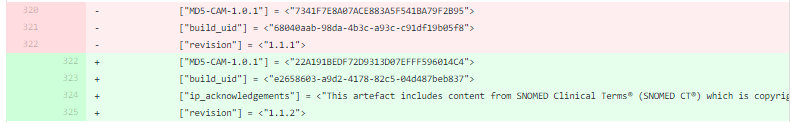
\includegraphics[width=1\textwidth]{img/compare_arch_versions.PNG}
	\caption{Values of archetype identification parameters modified after changes.}
	\label{fig:compare_arch_versions.PNG}
\end{figure}

\begin{figure}[H]
	\centering
  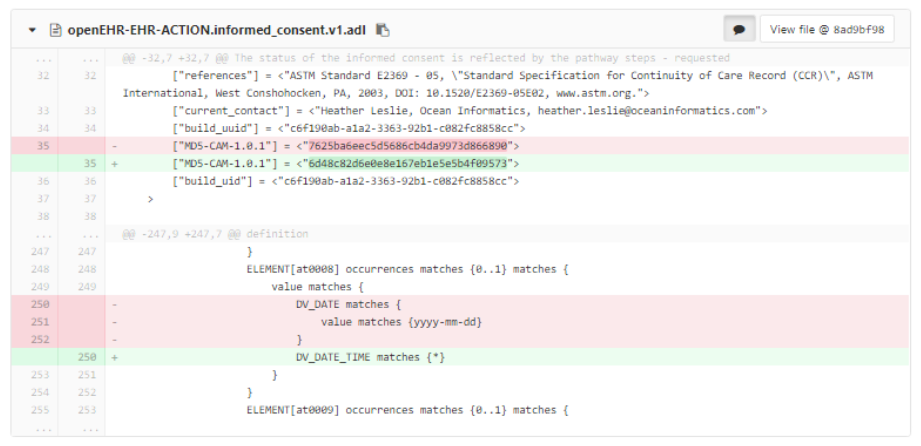
\includegraphics[width=1\textwidth]{img/MD5_hash_diff.PNG}
	\caption{Changing the archetype provoke modification on the MD5-CAM-1.0.1 hash}
	\label{fig:MD5_hash_diff}
\end{figure}

Some of these parameters, such as the "archetype\_UID", "Build\_UID" and "Canonical MD5 Hash" will be used to identify the new versions of archetypes in both repositories (international CKM and an local CKM) in the implementation and methodology chapters.


\textbf{Important note:} the cryptographic algorithms currently used to transform the archetypes identification and body into a hash string have already been broken by collisions attacks. This means that there is probability of an archetype to present the same hash of another different archetype (although it is a very small possibility to happen).


\section{Current outcomes from openEHR artifacts usage}
The goal of openEHR was creating a set of archetypes in a single international repository (openEHR CKM) that could be used in an EHR system after being agreed by the international online community. Was also possible to add regional or local archetypes that would still compatible with the previous ones inserted in the international CKM and making the information being shareable with everybody. However the current use of archetypes are not working in this way. 

Each project that makes use of archetypes have their own repository. Some of them are using the international CKM and being compliant with it. Other projects have download the archetypes from international CKM, but made a few changes on the archetype to reply to specification requirements (see section \ref{sssec:AS}) and then these are saved on local repositories like \textit{GitHub}, \textit{GitLab}, \textit{SubVersion} or \textit{Preforce}. This results in a jumble of archetypes variations from the international base of these archetypes, which was not the aim from openEHR. 

\section{Structure of openEHR Foundation International CKM Mirror on GitHub}
To maintain a copy of every artifact created on the openEHR CKM repository, the openEHR Foundation made a mirror from the international CKM and hosted it on GitHub. This mirror contains all the archetypes, templates and termsets from the CKM “Authoring TRUNK”, including the published and unpublished/unstable artifacts that keep going under active development and review. If the “Authoring TRUNK” from CKM changes, this behavior it is automatically replicated by this mirror repository on GitHub. 

The figure \ref{fig:CKM_mirror_organization} shows that currently the OpenEHR International CKM are divided in two main groups in the same blob (master): local and remote. The local group refers to all the artifacts (archetypes, templates and termsets) contained on the openEHR CKM (org.openehr) that were made and reviewed by the online community. The remote group refers to the other instances from CKM (Nehta, Nasjonalikt and UK Clinical Models) that have artifacts submitted to the main CKM, but still authored by them. Commonly the main CKM is the most complete of all the instances created after it. 

\begin{figure}[H]
	\centering
    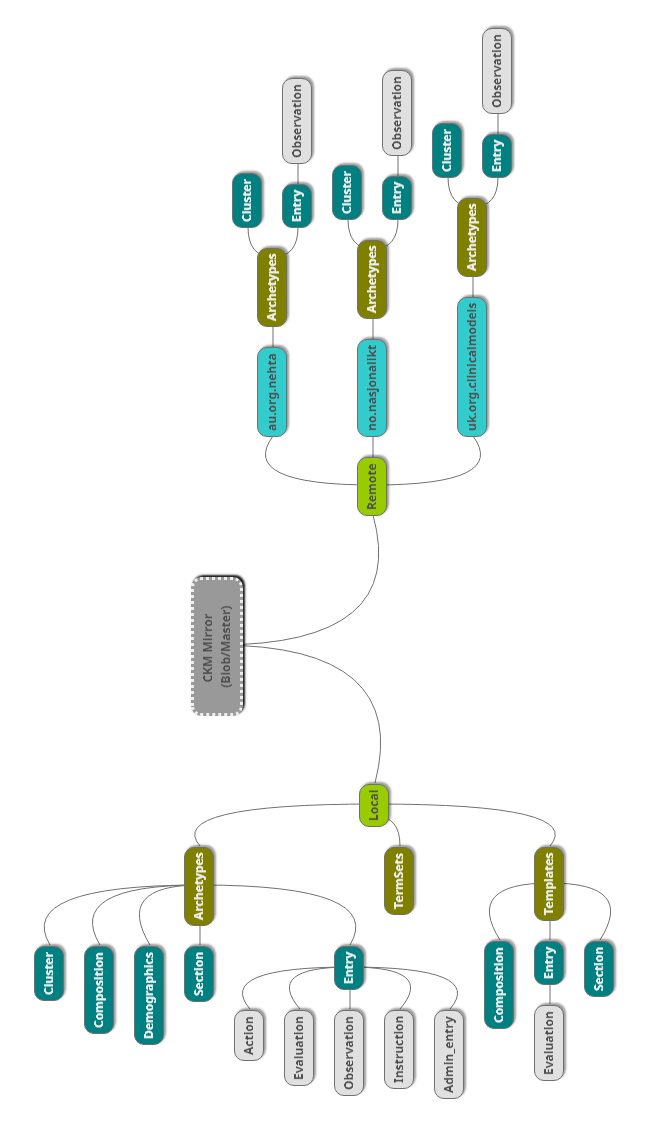
\includegraphics[width=0.9\textwidth]{img/CKM_mirror_organization.PNG}
	\caption{Structure of openEHR CKM mirror on GitHub (May 2018)}
	\label{fig:CKM_mirror_organization}
\end{figure}



\end{document}